% Options for packages loaded elsewhere
\PassOptionsToPackage{unicode}{hyperref}
\PassOptionsToPackage{hyphens}{url}
%
\documentclass[
  man]{apa6}
\usepackage{lmodern}
\usepackage{amssymb,amsmath}
\usepackage{ifxetex,ifluatex}
\ifnum 0\ifxetex 1\fi\ifluatex 1\fi=0 % if pdftex
  \usepackage[T1]{fontenc}
  \usepackage[utf8]{inputenc}
  \usepackage{textcomp} % provide euro and other symbols
\else % if luatex or xetex
  \usepackage{unicode-math}
  \defaultfontfeatures{Scale=MatchLowercase}
  \defaultfontfeatures[\rmfamily]{Ligatures=TeX,Scale=1}
\fi
% Use upquote if available, for straight quotes in verbatim environments
\IfFileExists{upquote.sty}{\usepackage{upquote}}{}
\IfFileExists{microtype.sty}{% use microtype if available
  \usepackage[]{microtype}
  \UseMicrotypeSet[protrusion]{basicmath} % disable protrusion for tt fonts
}{}
\makeatletter
\@ifundefined{KOMAClassName}{% if non-KOMA class
  \IfFileExists{parskip.sty}{%
    \usepackage{parskip}
  }{% else
    \setlength{\parindent}{0pt}
    \setlength{\parskip}{6pt plus 2pt minus 1pt}}
}{% if KOMA class
  \KOMAoptions{parskip=half}}
\makeatother
\usepackage{xcolor}
\IfFileExists{xurl.sty}{\usepackage{xurl}}{} % add URL line breaks if available
\IfFileExists{bookmark.sty}{\usepackage{bookmark}}{\usepackage{hyperref}}
\hypersetup{
  pdftitle={Relation between Shieh's delta and Cohen's delta},
  pdfauthor={Marie Delacre},
  pdfkeywords={keywords},
  hidelinks,
  pdfcreator={LaTeX via pandoc}}
\urlstyle{same} % disable monospaced font for URLs
\usepackage{graphicx,grffile}
\makeatletter
\def\maxwidth{\ifdim\Gin@nat@width>\linewidth\linewidth\else\Gin@nat@width\fi}
\def\maxheight{\ifdim\Gin@nat@height>\textheight\textheight\else\Gin@nat@height\fi}
\makeatother
% Scale images if necessary, so that they will not overflow the page
% margins by default, and it is still possible to overwrite the defaults
% using explicit options in \includegraphics[width, height, ...]{}
\setkeys{Gin}{width=\maxwidth,height=\maxheight,keepaspectratio}
% Set default figure placement to htbp
\makeatletter
\def\fps@figure{htbp}
\makeatother
\setlength{\emergencystretch}{3em} % prevent overfull lines
\providecommand{\tightlist}{%
  \setlength{\itemsep}{0pt}\setlength{\parskip}{0pt}}
\setcounter{secnumdepth}{-\maxdimen} % remove section numbering
\shorttitle{Shieh's delta vs. Cohen's delta}
\affiliation{
\vspace{0.5cm}
\textsuperscript{1} Université Libre de Bruxelles, Service of Analysis of the Data (SAD), Bruxelles, Belgium}
\keywords{keywords\newline\indent Word count: X}
\usepackage{csquotes}
\usepackage{upgreek}
\captionsetup{font=singlespacing,justification=justified}

\usepackage{longtable}
\usepackage{lscape}
\usepackage{multirow}
\usepackage{tabularx}
\usepackage[flushleft]{threeparttable}
\usepackage{threeparttablex}

\newenvironment{lltable}{\begin{landscape}\begin{center}\begin{ThreePartTable}}{\end{ThreePartTable}\end{center}\end{landscape}}

\makeatletter
\newcommand\LastLTentrywidth{1em}
\newlength\longtablewidth
\setlength{\longtablewidth}{1in}
\newcommand{\getlongtablewidth}{\begingroup \ifcsname LT@\roman{LT@tables}\endcsname \global\longtablewidth=0pt \renewcommand{\LT@entry}[2]{\global\advance\longtablewidth by ##2\relax\gdef\LastLTentrywidth{##2}}\@nameuse{LT@\roman{LT@tables}} \fi \endgroup}


\DeclareDelayedFloatFlavor{ThreePartTable}{table}
\DeclareDelayedFloatFlavor{lltable}{table}
\DeclareDelayedFloatFlavor*{longtable}{table}
\makeatletter
\renewcommand{\efloat@iwrite}[1]{\immediate\expandafter\protected@write\csname efloat@post#1\endcsname{}}
\makeatother
\usepackage{lineno}

\linenumbers

\title{Relation between Shieh's delta and Cohen's delta}
\author{Marie Delacre\textsuperscript{1}}
\date{}

\authornote{

Correspondence concerning this article should be addressed to Marie Delacre, CP191, avenue F.D. Roosevelt 50, 1050 Bruxelles. E-mail: \href{mailto:marie.delacre@ulb.ac.be}{\nolinkurl{marie.delacre@ulb.ac.be}}}

\abstract{

}

\begin{document}
\maketitle

\textbf{Cohen's \(\delta\)} is the difference between both groups means, divided by a pooled error term:

\begin{equation} 
Cohen's \; \delta= \frac{\mu_{1}-\mu_{2}}{\sqrt{\frac{(n_{1}-1) \times \sigma^2_{1} + (n_{2}-1) \times \sigma^2_{2}}{n_{1}+n_{2}-2}}}
\label{eq:cohend}
\end{equation}

\textbf{Shieh's \(\delta\)} is the difference between both groups means, divided by an unpooled error term (Shieh, 2013):

\begin{equation} 
Shieh's \; \delta= \frac{\mu_{1}-\mu_{2}} {\sqrt{\frac{\sigma_1^2}{n_1/N}+\frac{\sigma_2^2}{n_2/N}}}
\label{eq:shiehs}
\end{equation}

Unlike the classical Cohen's \(\delta\), Shieh's \(\delta\) depends on the sample size ratio (i.e.~\(\frac{n_1}{n_2}\) that I will call later nratio). For the same amount of differences between two means, same standard deviations and \(\sigma\)-ratio, Shieh's \(\delta\) will vary as a function of the nratio. Shieh's \(\delta\) can therefore be expressed as a function of the nratio:

\begin{equation} 
Shieh's \; \delta= \frac{(\mu_1-\mu_2) \times \sqrt{nratio}}{(nratio+1) \times \hat{\sigma}},\hat{\sigma} = \sqrt{(1-\frac{n_1}{N}) \times \sigma_1^2+(1-\frac{n_2}{N}) \times \sigma_2^2}
\label{eq:shieh}
\end{equation}

To illustrate the relation between Shieh's \(\delta\) and the nratio, we can calculate the parameter across a range of nratio. We will first study the Shieh's \(\delta\) (and its relation with Cohen's \(\delta\)) when variances are equal between groups. We will then go through the relation when variances are unequal between groups.

\hypertarget{when-variances-are-equal-between-groups}{%
\section{When variances are equal between groups}\label{when-variances-are-equal-between-groups}}

As a first example, in Figure \ref{fig:SHIEH1}, Cohen's \(\delta\) and Shieh's \(\delta\) are calculated for different configurations where the observed mean difference (\(\mu_{1}-\mu_{2}\)) is 1, the total sample size is 200 and standard deviations \(\sigma_{1}\) and \(\sigma_{2}\) both equals 2\footnote{Note that we chose a mean difference of 1 for convenience, however the mean difference does not impact the relation between both effect size measures}.

First, when sample sizes are equal across groups, one can observe that Shieh's \(\delta\) is half of the value of Cohen's \(\delta\). Shieh's \(\delta\) equals 0.25 when nratio is 1, and Cohen's \(\delta\) equals 0.50:

\begin{equation} 
Shieh's \; \delta_{n_1=n_2} = \frac{Cohen's \; \delta_{n_1=n_2}}{2}
\leftrightarrow Shieh's \; \delta_{n_1=n_2}= \frac{\mu_1-\mu_2}{2 \times \hat{\sigma}} 
\label{eq:cohenshieh}
\end{equation}

Note that when variances are equal between groups, Cohen's \(\delta\) is constant whatever groupe sample sizes are equal or not (i.e.~Cohen's \(\delta_{n1=n2}\) = Cohen's \(\delta_{n1 \neq n2}\)). This equality will no longer be true when variances are unequal between groups. We use therefore \(\delta_{Cohen, n_1=n_2}\) in Formula \ref{eq:cohenshieh}, in order that equality is still applicable when variances are unequal between groups (see later).

Moreover, when both sample sizes are equal between groups, Shieh's \(\delta\) achieves its maximum value. When plotting both parameters against the log of the nratio, one can more easily observe that the Shieh's \(\delta\) departs symmetrically from it's maximum value as long as the nratio moves away from 1 (i.e.~when log(nratio) = 0; see Figure \ref{fig:SHIEH2}).

When variances are equal between groups, \(\hat{\sigma}\) will be the same for all nratio (\(\hat{\sigma}=\sigma_1=\sigma_2\); i.e.~\(\hat{\sigma}\) in Equation \ref{eq:shieh} = \(\hat{\sigma}\) in Equation \ref{eq:cohenshieh}), one can deduce that the relation between Shieh's \(\delta\) value when nratio=1 and its value for all other nratio can be expressed as follows:

\begin{equation} 
Shieh's \; \delta_{n_1=n_2} = Shieh's \; \delta \times \frac{\frac{\mu_1-\mu_2}{2 \times \hat{\sigma}}}{\frac{(\mu_1-\mu_2) \times \sqrt{nratio}}{(nratio+1) \times \hat{\sigma}}}
\leftrightarrow Shieh's \; \delta_{n_1=n_2} = Shieh's \; \delta \times \frac{nratio+1}{2 \times \sqrt{nratio}}
\label{eq:shiehvsmax}
\end{equation}

Note that because of formula \ref{eq:cohenshieh} and because we know that Cohen's \(\delta\) is constant for all nratio, when variances are equal between groups, one can conclude that the relation between Cohen's \(\delta\) and Shieh's \(\delta\) can be expressed as following:

\begin{equation} 
Cohen's \; \delta_{n_1=n_2}= Shieh's \; \delta \times \frac{nratio+1}{\sqrt{nratio}}
\label{eq:shiehvsmax}
\end{equation}

This relations remains true as long as variances are equal between groups.

\begin{figure}
\centering
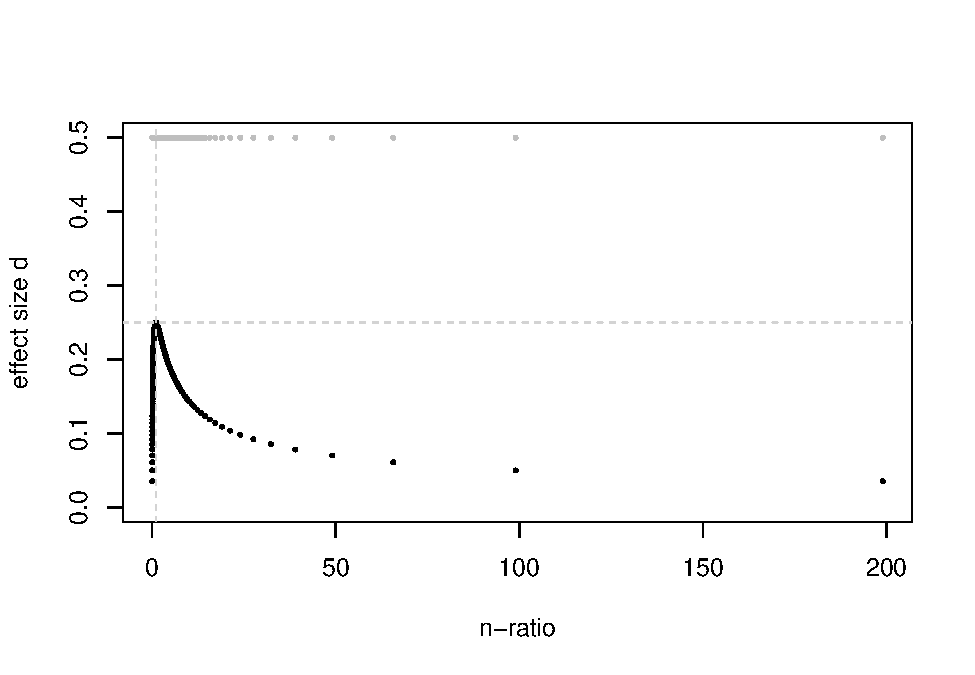
\includegraphics{Appendix1_files/figure-latex/SHIEH1-1.pdf}
\caption{\label{fig:SHIEH1}Comparison of Shieh's d (black dots) and Cohen's d (grey dots) when mu1 - mu2 = 1, N = 200 and sigma 1 and sigma 2 both equals 2}
\end{figure}

\begin{figure}
\centering
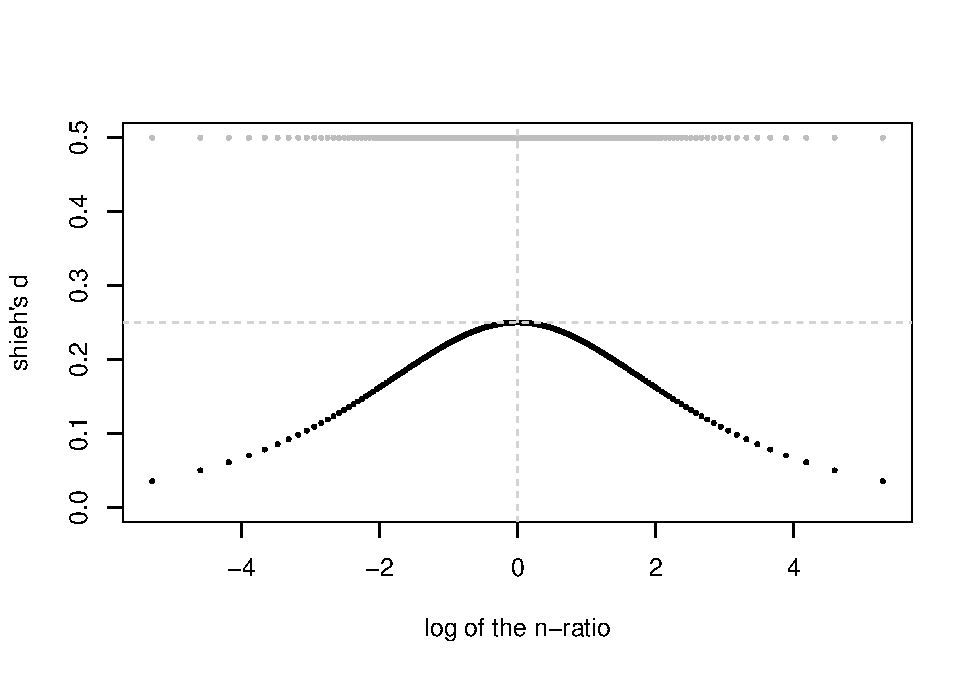
\includegraphics{Appendix1_files/figure-latex/SHIEH2-1.pdf}
\caption{\label{fig:SHIEH2}Comparison of Comparison of Shieh's d (black dots) and Cohen's d (grey dots) when mu1 - mu2 = 1, N = 200 and delta 1 = delta 2 = 2}
\end{figure}

\hypertarget{when-variances-are-unequal-between-groups}{%
\section{When variances are unequal between groups}\label{when-variances-are-unequal-between-groups}}

In Figure \ref{fig:SHIEH3}, Cohen's \(\delta\) and Shieh's \(\delta\) are calculated for different configurations where the observed mean difference (\(\mu_{1}-\mu_{2}\)) is 1, the total sample size is 200 and standard deviations \(\sigma_{1}\) and \(\sigma_{2}\) are respectively 4 and 3 (left) or 3 and 4 (right). As one can see, when variances are unequal between groups, Cohen's \(\delta\) no longer remains constant for all nratio.

\begin{figure}
\centering
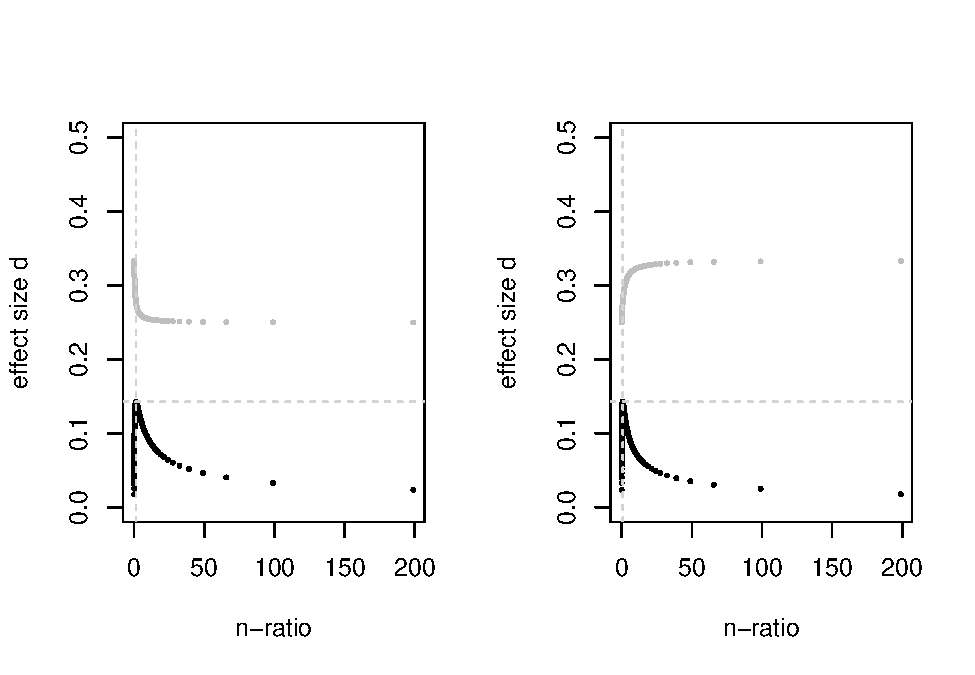
\includegraphics{Appendix1_files/figure-latex/SHIEH3-1.pdf}
\caption{\label{fig:SHIEH3}Comparison of Shieh's d (black dots) and Cohen's d (grey dots) when mu1 - mu2 = 1, N = 200 and sigma 1 and sigma 2 are respectively 4 and 2 (left) or 2 and 4 (right)}
\end{figure}

Once again, it is easier to study the influence of the nratio on both parameters when plotting them against the log of the nratio, as done in Figure \ref{fig:SHIEH4}.
The way the standard error term is computed in Cohen's \(\delta\) (see formula \ref{eq:cohend}) implies that all samples are considered as issued from a common population variance (hence the assumption of homoscedasticity). When there is heteroscedasticity, if the larger variance is associated with the larger sample size (i.e.~the colored parts on both plots in Figure \ref{fig:SHIEH4}), the error term is overestimated and therefore, the Cohen's \(\delta\) is decreased. The smallest value is achieved when the sample size of the group associated with the largest variance equals n-1=199 (i.e.~when one gives the largest weight to the largest standard deviation). On the other side, if the larger variance is associated with the smaller sample size (i.e.~the non-colored parts of both plots), the error term is underestimated and therefore, the Cohen's \(\delta\) is increased. The largest value is achieved when the sample size of the group associated with the largest variance equals 1 (i.e.~when one gives the largest weight to the smallest standard deviation).

Unlike Cohen's \(\delta\), Shieh's \(\delta\) is not influenced by the correlation between the sample size and the standard deviation.

While it remains true that when \(n_{1}=n_{2}\), the Cohen's \(\delta\) is exactly as twice as large as Shieh's \(\delta\) (Shieh's \(\delta\) equals 0.25 and Cohen's \(\delta\) equals 0.50), the maximum Shieh's \(\delta\) value is no longer when the nratio equals 1 (i.e the log of the nratio equals 0). Moreover, Shieh's \(\delta\) no longer departs symmetrically from it's maximum value as a function of the nratio. This is due to the fact that \(\hat{\sigma}\) will vary a function of the nratio (and will therefore be different for all configurations presented in Figure \ref{fig:SHIEH4}): as shown in formula \ref{eq:shieh}, one gives more weight to the standard deviation associated with the smallest group. For this reason, the maximum Shieh's \(\delta\) is always achieved when there is a positive correlation between variances and sample sizes (i.e.~we give more weight to the smallest standard deviation, associated with the smallest group) and the more unequal the variances, the further from 1 the nratio associated with the maximum , as illustrated in Figure \ref{fig:SHIEH5}.

As a consequence of different \(\hat{\sigma}\) for all nratio's, the relation between Shieh's \(\delta\) value when nratio=1 and its value for all other nratio cannot be as simplifed as it was when variances were equal:

\begin{equation} 
Shieh's \; \delta_{n_1=n_2}= Shieh's \; \delta \times \frac{\frac{\mu_1-\mu_2}{2 \times \sigma_{(n_1=n_2)}}}{\frac{(\mu_1-\mu_2) \times \sqrt{nratio}}{(nratio+1) \times \sigma_{(n_1\neq n_2)}}}
\leftrightarrow Shieh's \; \delta_{n_1=n_2}= Shieh's \; \delta \times \frac{(nratio+1) \times \sigma_{n_1 \neq n_2}}{2 \times \sigma_{n_1=n_2} \times \sqrt{nratio}}
\label{eq:shiehvsbaldesign}
\end{equation}

With \[\sigma_{n_1=n_2}= \sqrt{\frac{\sigma_1^2+\sigma_2^2}{2}}\] and
\[\sigma_{n_1 \neq n_2} = \sqrt{(1- \frac{n_1}{N}) \times \sigma_1^2+(1- \frac{n_2}{N}) \times \sigma_2^2}\]

Finally, because of formula \ref{eq:cohenshieh}, one can conclude that the relation between the Cohen's \(\delta\) we would obtain if sample sizes were equal between groups and Shieh's \(\delta\) can be expressed as following:

\begin{equation} 
Cohen's \; \delta{n_1=n_2}= Shieh's \; \delta \times \frac{(nratio+1) \times \sigma_{n_1 \neq n_2}}{\sigma_{n_1=n_2} \times \sqrt{nratio}}
\label{eq:shiehvsbaldesign2}
\end{equation}

Formula \ref{eq:shiehvsbaldesign2} gives us the general relation between Shieh's \(\delta\) and Cohen's \(\delta\),applicable whatever variances are equal between groups or not.

\begin{figure}
\centering
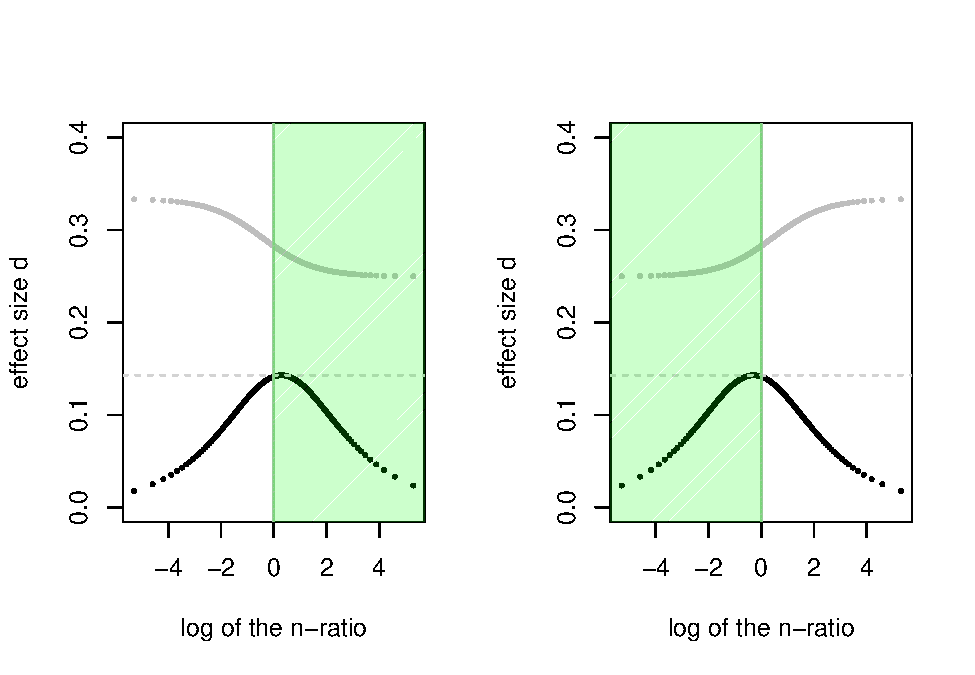
\includegraphics{Appendix1_files/figure-latex/SHIEH4-1.pdf}
\caption{\label{fig:SHIEH4}Comparison of Shieh's d (black dots) and Cohen's d (grey dots) when mu1 - mu2 = 1, N = 200 and sigma 1 and sigma 2 are respectively 4 and 2 (left) or 2 and 4 (right)}
\end{figure}

\begin{figure}
\centering
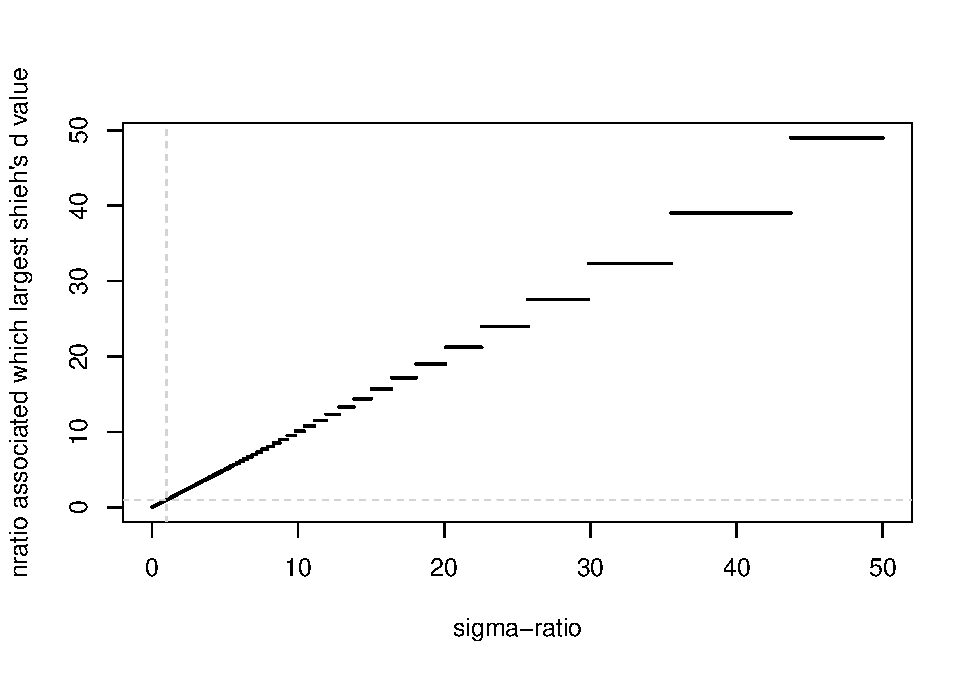
\includegraphics{Appendix1_files/figure-latex/SHIEH5-1.pdf}
\caption{\label{fig:SHIEH5}At which nratio the largest value of Shieh's d is achieved, as a function of the sigma-ratio (= sigma1/sigma2)}
\end{figure}

\begin{figure}
\centering
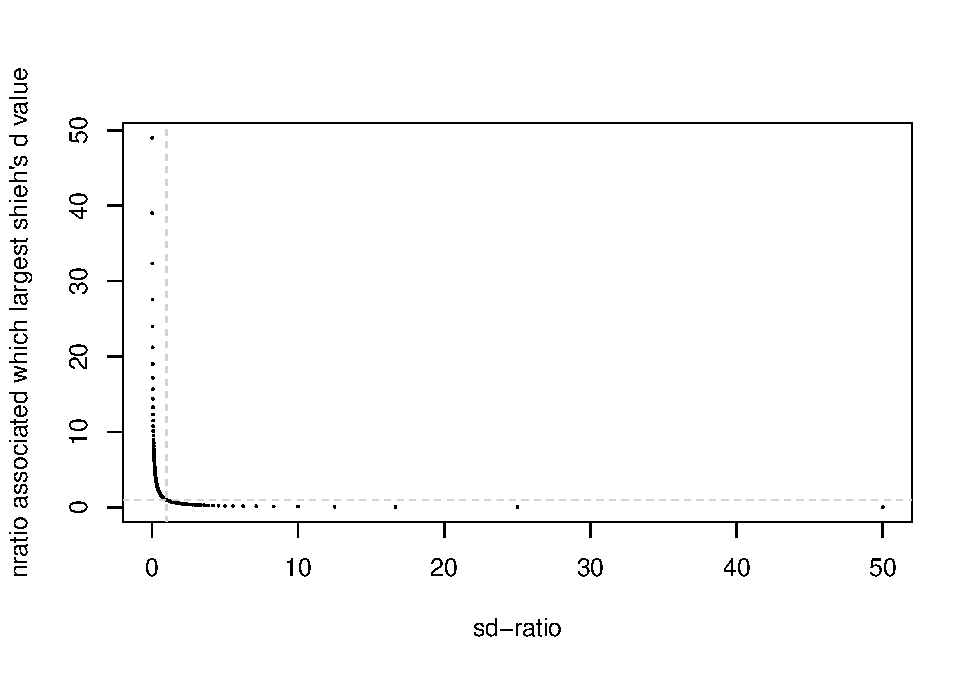
\includegraphics{Appendix1_files/figure-latex/SHIEH6-1.pdf}
\caption{\label{fig:SHIEH6}At which nratio the largest value of Shieh's d is achieved, as a function of the sigma-ratio (= sigma1/sigma2)}
\end{figure}

\end{document}
